\documentclass[final]{siamltex}

% for red MarginPars
\usepackage{color}

\usepackage{epsfig}
\usepackage{bm}

% total number of floats allowed on a page
\setcounter{totalnumber}{100}

% float page fractions
\renewcommand{\topfraction}{0.9}
\renewcommand{\bottomfraction}{0.9}
\renewcommand{\textfraction}{0.2}

% MarginPar
\setlength{\marginparwidth}{0.75in}
\newcommand{\MarginPar}[1]{\marginpar{\vskip-\baselineskip\raggedright\tiny\sffamily\hrule\smallskip{\color{red}#1}\par\smallskip\hrule}}

\def\eb  {{\bf e}}
\def\ib  {{\bf i}}
\def\nb  {{\bf n}}
\def\mRb {\bm{\mathcal{R}}}
\def\mZb {\bm{\mathcal{Z}}}

\def\half   {\frac{1}{2}}
\def\myhalf {\sfrac{1}{2}}

% for non-stacked fractions
\newcommand{\sfrac}[2]{\mathchoice
  {\kern0em\raise.5ex\hbox{\the\scriptfont0 #1}\kern-.15em/
   \kern-.15em\lower.25ex\hbox{\the\scriptfont0 #2}}
  {\kern0em\raise.5ex\hbox{\the\scriptfont0 #1}\kern-.15em/
   \kern-.15em\lower.25ex\hbox{\the\scriptfont0 #2}}
  {\kern0em\raise.5ex\hbox{\the\scriptscriptfont0 #1}\kern-.2em/
   \kern-.15em\lower.25ex\hbox{\the\scriptscriptfont0 #2}}
  {#1\!/#2}}

\begin{document}

%==========================================================================
% Title
%==========================================================================
\title{User's Guide to Stochastic Diffusion/Reaction Code}

\maketitle

\section{Introduction}
This is a working design document for our stochastic diffusion/reaction code.
In summary, we are solving the following system of stochastic PDEs:
\begin{equation}
\frac{\partial n_k}{\partial t} = \nabla\cdot\left(D_k\nabla n_k + \sqrt{2D_kn_k}\mZb\right) + \mRb(\nb),
\end{equation}
where $\nb=(n_1,n_2,\cdots)$ are the number densities, $D_k$ are Fickean diffusion
coefficients, and $\mZb$ are standard zero-mean, unit-variance random Gaussian 
vector fields with uncorrelated components.
This model is essentially the fluctuating multispecies diffusion equations
augmented with a stochastic reaction term, $\mRb$.

\section{Source Code}
There are two git repositories required to build/run the code.  BoxLib is a public
repository available on github using the command:\\ \\
{\tt git clone https://github.com/BoxLib-Codes/BoxLib.git}\\ \\
If you are not familiar with BoxLib, we recommend reading the BoxLib's User's Guide
in {\tt BoxLib/Docs}.\\

FluctHydro exists on CCSE servers and you need to contact Vince/Andy to get an account
and set up permissions on gamera.  Once you do, you can obtain the repository using:\\ \\
{\tt git clone <username>@gamera.lbl.gov:/usr/local/gitroot/FluctHydro.git}\\ \\
You will now have the following directory structures (you will actually have
more subdirectories, but below are the only directories that matter for this code):\\
%%%%%%%%%%%%%%%%%%%%%%%%%%%%%%%%%%%%%
\begin{figure}[tb]
\centering
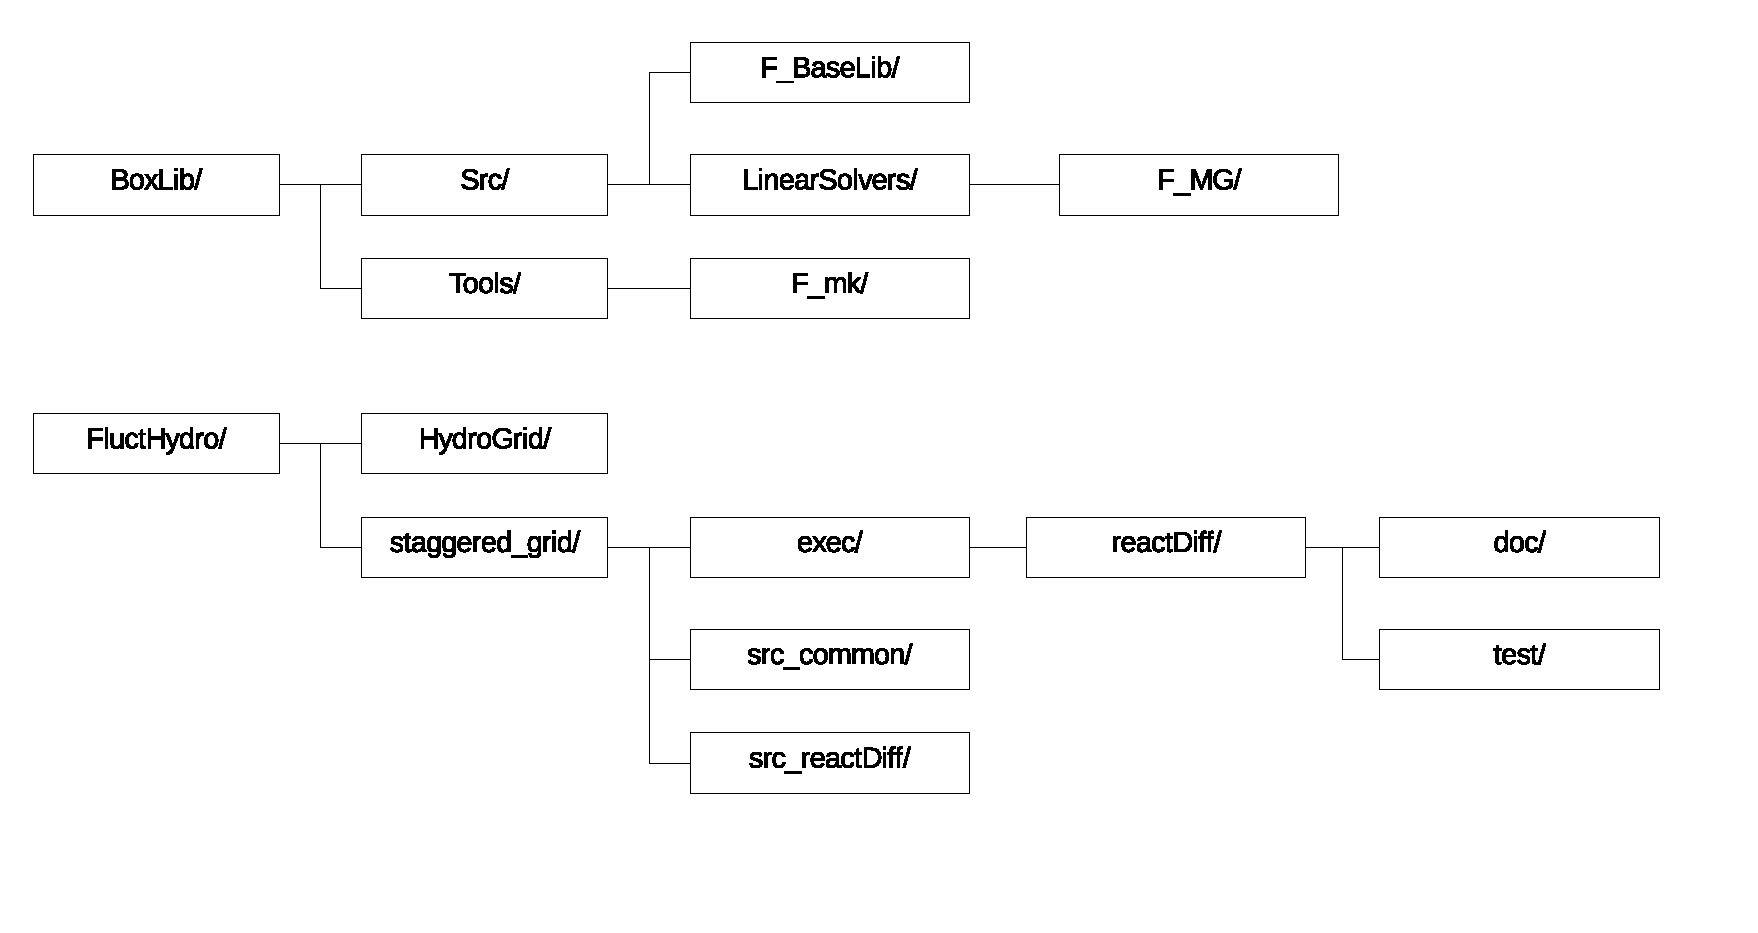
\includegraphics[width=6in]{./directory}
\caption{\label{fig:directory}Directory structure.}
\end{figure}
%%%%%%%%%%%%%%%%%%%%%%%%%%%%%%%%%%%%%
\begin{itemize}

\item {\tt BoxLib/}

\begin{itemize}

\item {\tt Src/}

\begin{itemize}

\item {\tt F\_BaseLib/}

Core libraries for parallelization of structured grid data.

\item {\tt LinearSolvers/F\_MG/}

Core libraries for linear solvers (for implicit diffusion) and diffusion stencils.

\end{itemize}
\end{itemize}

\begin{itemize}

\item {\tt Tools/F\_mk/}

Make system variables and flags.

\end{itemize}
\end{itemize}

\begin{itemize}

\item {\tt FluctHydro/}

\begin{itemize}

\item {\tt HydroGrid/}

\item {\tt staggered\_grid/}

\begin{itemize}

\item {\tt exec/reactDiff/doc/}

Contains the document you are reading right now!

\item {\tt exec/reactDiff/test/}

This is the compilation directory.  Contains a GNUmakefile and inputs files.

\item {\tt src\_common/}

Source code shared by all our staggered grid codes.  Contains generic namelist parameters
and routines for boundary conditions, divergence, etc.

\item {\tt src\_reactDiff/}

Source code specific to this reaction/diffusion problem.

\end{itemize}
\end{itemize}
\end{itemize}

\subsection{Compiling and Running}
Go to {\tt FluctHydro/staggered\_grid/exec/reactDiff/test/} and edit the 
{\tt GNUmakefile} settings to your liking (below) and simply type {\tt `make'}.\\
\begin{verbatim}
NDEBUG    :=           # 'not debug'.  use 't' for an optimized build
MPI       := t         # use 't' to build an mpi executable
OMP       :=           # use 't' to build an OpenMP threadded executable
PROF      :=           # use 't' to turn on code profiling
COMP      := gfortran  # fortran compiler
CCOMP     := gcc       # c compiler
MKVERBOSE := t         # make verbosity

\end{verbatim}
This will generate an executable whose name provides information about the build settings,
i.e., what compiler was used, whether MPI and/or OpenMP were enabled, etc.
To run the code, simply type the executable name, followed by an inputs file.

\subsection{Input Parameters}
Refer to {\tt src\_common/probin\_common.f90} and 
{\tt src\_reactDiff/probin\_reactDiff.f90} for namelist parameters used in the
simulation and an explanation of what the parameters do.  Note that only a subset
of the parameters in {\tt probin\_common.f90} are used in this code.

\section{Algorithm}
We use a finite volume framework on a regular Cartesian mesh.  Consider PDEs describing
diffusion and reactions in isolation:
\begin{equation}
\frac{\partial n_k}{\partial t} = \nabla\cdot\left(D_k\nabla n_k + \sqrt{2D_kn_k}\mZb\right),\label{eq:Diffusion}
\end{equation}
\begin{equation}
\frac{\partial n_k}{\partial t} = \mRb(\nb).\label{eq:Reactions}
\end{equation}
The code supports three temporal splitting schemes:\\

{\bf First-Order Temporal Splitting}
\begin{enumerate}
\item Advance $\nb^n \rightarrow \nb^{(1)}$ by discretizing 
(\ref{eq:Diffusion}) over $\Delta t$.
\item Advance $\nb^{(1)} \rightarrow \nb^{n+1}$ by discretizing 
(\ref{eq:Reactions}) over $\Delta t$.
\end{enumerate}

{\bf Second-Order Strang Splitting, Option 1}
\begin{enumerate}
\item Advance $\nb^n \rightarrow \nb^{(1)}$ by discretizing 
reactions (\ref{eq:Reactions}) over $\Delta t/2$.
\item Advance $\nb^{(1)} \rightarrow \nb^{(2)}$ by discretizing 
diffusion (\ref{eq:Diffusion}) over $\Delta t$.
\item Advance $\nb^{(2)} \rightarrow \nb^{n+1}$ by discretizing 
reactions (\ref{eq:Reactions}) over $\Delta t/2$.
\end{enumerate}

{\bf Second-Order Strang Splitting, Option 2}
\begin{enumerate}
\item Advance $\nb^n \rightarrow \nb^{(1)}$ by discretizing 
diffusion (\ref{eq:Diffusion}) over $\Delta t/2$.
\item Advance $\nb^{(1)} \rightarrow \nb^{(2)}$ by discretizing 
reactions (\ref{eq:Reactions}) over $\Delta t$.
\item Advance $\nb^{(2)} \rightarrow \nb^{n+1}$ by discretizing 
diffusion (\ref{eq:Diffusion}) over $\Delta t/2$.
\end{enumerate}

\subsection{Diffusion}
The Fickean diffusion term is discretized using standard finite volume
Laplacian-like stencils:
\begin{equation}
\nabla\cdot D\nabla n \rightarrow \sum_d \frac{1}{\Delta x}\left[D_{\ib+\half\eb_d}\left(\frac{n_{\ib + \eb_d}-n_{\ib}}{\Delta x}\right) - D_{\ib-\half\eb_d}\left(\frac{n_{\ib}-n_{\ib-\eb_d}}{\Delta x}\right)\right],\label{eq:diffusion_stencil}
\end{equation}
For the stochastic fluxes,
we generate random $\mZb$ on faces directory, compute $n$ on faces
using either arithmetic, geometric, or harmonic averaging from the 
neighboring cell centers, and use the same stencil 
in (\ref{eq:diffusion_stencil}).\\

In order to discretize the diffusion equation (\ref{eq:Diffusion}) over a time 
increment $\delta t$, we have three options.  We use the superscripts $n$
and $n+1$ to denote the state at $t^n$ and $t^{n+1}=t^n+\delta t$, noting
that $\delta t$ can be a fraction of the time step $\Delta t$.\\

{\bf Explicit Predictor-Corrector}
We use a single set of random numbers, and keep the noise amplitude
fixed (Ito interpretation):
\begin{equation}
n_k^{n+1,*} = n_k^n + \delta t \nabla\cdot\left(D_k \nabla n_k^n
+ \sqrt{\frac{2 D_k n_k^n}{\delta t\Delta V}}\mZb^{(1)}\right),
\end{equation}
\begin{equation}
n_k^{n+1} = n_k^n + \delta t\left(
\half D_k\nabla n_k^n + \half D_k\nabla n_k^{n+1,*}
+ \sqrt{\frac{2 D_k n_k^n}{\delta t\Delta V}}\mZb^{(1)}
\right).
\end{equation}

{\bf Crank-Nicolson}
We update the number densities using a single semi-implicit solve:
\begin{equation}
n_k^{n+1} = n_k^n + \delta t\left(
\half D_k\nabla n_k^n + \half D_k\nabla n_k^{n+1}
+ \sqrt{\frac{2 D_k n_k^n}{\delta t\Delta V}}\mZb^{(1)}
\right).
\end{equation}

{\bf Explicit Midpoint}
We use two sets of random numbers, but use the same noise amplitude for both:
\begin{equation}
n_k^{n+\myhalf} = n_k^n + \frac{\delta t}{2} \nabla\cdot\left(D_k\nabla n_k^n
+ \sqrt{2}\sqrt{\frac{2 D_k n_k^n}{\delta t\Delta V}}\mZb^{(1)}\right),
\end{equation}
\begin{equation}
n_k^{n+1} = n_k^n + \delta t\left(
D_k\nabla n_k^{n+\myhalf}
+ \sqrt{2}\sqrt{\frac{2 D_k n_k^n}{\delta t\Delta V}}\left(\mZb^{(1)}+\mZb^{(2)}\right)
\right).
\end{equation}

\subsection{Reactions}
In order to discretize the reaction equation (\ref{eq:Reactions}) over a time
increment $\delta t$, we have three options: stochastic
simulation algorithm (SSA), tau-leaping, and chemical Langevin equation (CLE).
See \cite{Gillespie2007} for an overview of these methods.  We have options
for second-order tau-leaping and CLE using the predictor-corrector
method in \cite{AndersonMattingly2011}.\\

Our stochastic reactions require deterministic reaction rates, which we obtain
using the law of mass action.  Define $a_i(\nb)$ as the deterministic reaction
rate in units of (?) for reaction $i$, and $a_0(\nb) = \sum a_i(\nb)$.\\

{\bf SSA}.  To summarize, if we assume each reaction is a Poisson process, we
can generate the time that the next reaction will occur using a uniform random
variable, and then determine which reaction occurred using a separate 
uniform random variable.  Then, update the state and repeate.\\

{\bf Tau Leaping}\\

{\bf CLE}

\bibliographystyle{plain}
\bibliography{DesignDocument}

\end{document}
